\chapter{Layout Languages as Sugared Attribute Grammars}
\section{Motivation and Approach}

We start by examining the concerns in building layout languages and our approach to addressing them by using and extending the attribute grammar formalism.  Throughout this and the remaining chapters, we focus on the design and implementation of one simple layout widget. We will show how our support of it generalizes to common layout languages and, more generally, computations over trees.

\subsection{Important properties for layout languages and others}
Layout languages are an important part of computing -- for one gauge, there are over 634 million websites live in 2012, with 51 million added that year~\footnote{http://news.netcraft.com/archives/2012/12/04/december-2012-web-server-survey.html}. Beyond the CSS and HTML languages for webpage layout, there are also \LaTeX~[[CITE]] for document layout, D3~[[CITE]] for data visualization, Swing~[[Swing]] for GUI layout, and even specialities within these domains such as markdown for text. 


Popular layout languages provide many sophisticated abstractions to foster designer productivity.
The alternative of asking a designer to manually specify for each element its position on a canvas and the style is analogous to asking a programmer to write in a low-level language such as assembly. Instead, layout languages resemble constraint systems where designers  declare high-level properties such as, in the program \code{hello world}, the words \code{hello} and \code{world} should be rendered, and with word \code{world} following line-wrapping rules for its positioning after \code{hello}. Layout languages may provide quite complicated constraints -- for example, most document layout languages define their rule line wrapping rule through an implementation in  a low-level language. Likewise, the constraints can be quite numerous, such as in the 250+ pages of rules for the CSS language. Adding to the sophistication, designers can often add their own constraints, such as through macros in \LaTeX,  percentage constraints in CSS, and arbitrary functions in Adobe Flex~[[CITE]]. 

The richness of popular layout languages comes at the cost of broad challenges in their design and implementation:

\begin{itemize}
\item \textbf{Safe semantics.} Does every input layout have exactly one unique rendering? Are the constraints restricted enough that an efficient implementation is feasible for low-power devices, big data sets, or fast animation? When a feature is added, does it conflict with anything of the above properties? We want a way to verify such properties.
\item \textbf{Safe implementation.} As a layout language grows in popularity, it grows in features. Likewise, developers will port it to many platforms and optimize it, and in cases such as CSS, reimplement it from scratch. Does the implementation conform to the intended semantics? Conformance bugs for CSS plague developers~[[CITE]], and failures to match {\LaTeX}'s semantics have killed multiple attempts to modernize the implementation. We want a way to verify that the implementation matches the specification.
\item \textbf{Advanced implementation.} Layout languages tend to add feature as they evolve. However, the implementation of each feature also has demands that increase with time: improved speed and memory footprint, better debugging support, etc. Browser layout engines for CSS are currently over 100,000 lines of optimized C++ code, and most rich layout languages thus far have resisted parallelization. We want automation techniques to assuage the implementation burden and more aggressively target those goals.
\end{itemize}


\begin{figure}
\centering
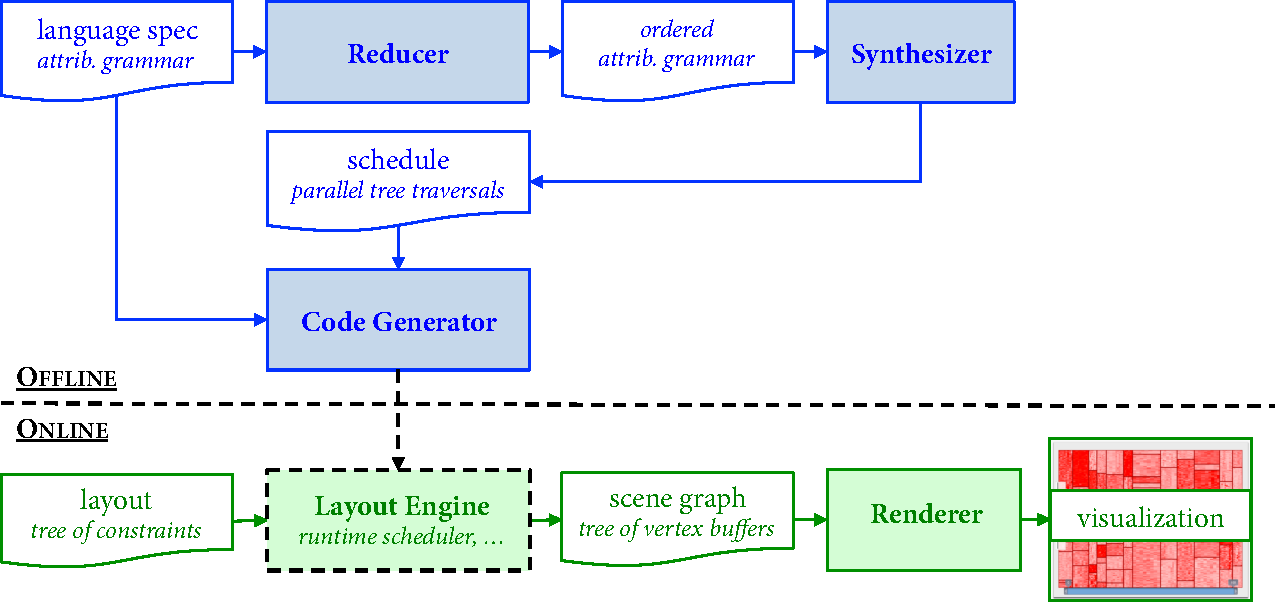
\includegraphics[trim=0 0 0 0,clip,width=1.0\columnwidth]{chapter2/architecture}
\caption{\textbf{Layout engine architecture.} }
\label{fig:architecture}
\end{figure}

Our idea is to define layout languages with an attribute grammar formalism that supports automated reasoning and program transformation. We show that the attribute grammar formalism supports specification of layout languages. It is unclear how to do so with the traditional attribute grammar formalism, so we support difficult cases of layout languages in a high-level form of attribute grammars and reduce reasoning about them to handling a more traditional formalism. The remainder of this chapter introduces the high-level attribute grammar formalism, how to specify layout languages using it, and an intuition for the reduction into a lower-level formalism. Figure~\ref{fig:architecture} depicts our architecture, including the split between offline generation of the layout engine and then how it is used at runtime to process a layout.



\section{The HBox Language as a Classical Attribute Grammar}
\subsection{Example tree with dynamic dependencies}
\subsection{Example static grammar instance}
\subsection{Dynamic evaluator}

\section{Desugaring Loops and Other Modern Constructs}
\subsection{Motivation: Productive Features with Simple Implementations}
\subsection{Interfaces: Lightweight and Reusable Input/Output Specifications}
\subsection{Traits: Reusing Cross-cutting Code}
\subsection{Loops}
\subsection{Embedded Domain Specific Language: Functional Rendering}



\section{Evaluation: Mechanized Layout Features}





\subsection{Rendering: Immediate Mode and Beyond}
\subsection{Non-euclidean: Sunburst Diagram}
\subsection{Charts: Line graphs}
\subsection{Animation and Interaction: Treemap}
\subsection{Flow-based: CSS Box Model}
\subsection{Grid-based: HTML Tables}

\section{Related Work}
\begin{itemize}
\item loose formalisms: browser impl (C++), d3 (JavaScript), latex formulas (ML)
\item restricted formalisms: cassowary and hp, UREs
\item AGs: html tables
\end{itemize}



